\documentclass[aspectratio=169,12pt]{beamer}

%\includeonlyframes{current}

\usepackage[utf8]{inputenc}
\usepackage[american]{babel}
\usepackage{amsmath,amsthm}
\usepackage{unicode}
\usepackage{booktabs}
\usepackage{ifthen}
\usepackage{tikz}
\usetikzlibrary{calc,arrows,positioning,patterns,decorations.pathmorphing}
\usepackage{ulem}

\mode<presentation>{%
  \usetheme{ibm}
}

\newcommand{\Z}{ℤ}
\newcommand{\F}{\mathbb{F}}
\renewcommand{\a}{\mathfrak{a}}
\renewcommand{\b}{\mathfrak{b}}
\newcommand{\g}{\mathfrak{g}}
\newcommand{\G}{\mathcal{G}}
\newcommand{\E}{\mathcal{E}}
\newcommand{\End}{\operatorname{End}}
\newcommand{\Hom}{\operatorname{Hom}}
\newcommand{\M}{\mathcal{M}}
\newcommand{\fp}{\mathrm{fp}}
\DeclareMathOperator{\rank}{rank}
\newcommand{\Cl}{\operatorname{Cl}}
\newcommand{\GL}{\operatorname{GL}}
\newcommand{\SL}{\operatorname{SL}}
\renewcommand{\O}{\mathcal{O}}

\title{Not Again!}
\subtitle{What's going on in isogeny-based crypto?}
\author{Luca De Feo}
\date[August 12, 2026, AMPQC, Ohrid]{August 12, 2026, Algebraic Methods in Post-quantum Cryptography, Ohrid}
\institute{IBM Research Zürich}

\begin{document}

\frame[plain]{\titlepage}

%%

\begin{frame}{A group}
  \Large
  \begin{center}
    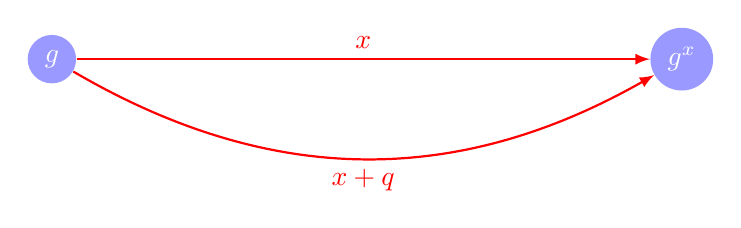
\begin{tikzpicture}
      \path[every node/.style={circle,white,fill=blue!40!white}]
      (0,0) node (E) {$g$}
      (8,0) node (E1) {$g^x$};
      \draw[-latex,red,thick] (E) edge node[above] {$x$} (E1);
      \uncover<2->{
        \draw[-latex,red,thick] (E) edge[bend right] node[below] {$x+q$} (E1);
      }
    \end{tikzpicture}
  \end{center}
\end{frame}

%%

\begin{frame}{Several generators}
  \centering\Large
  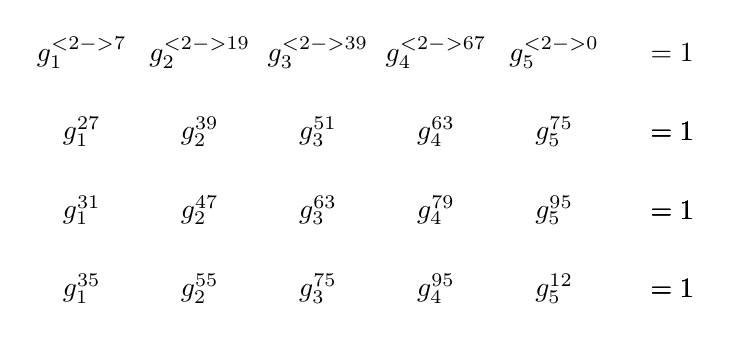
\begin{tikzpicture}[xscale=1.5]
    \foreach  \i in {1,...,5} {
      \pgfmathtruncatemacro\e{mod(313*\i*\i+3, 103)}
      \node at (\i, 0) {$g_\i^{\uncover<2->{\e}}$};
    }
    \uncover<2->{
      \node at (6, 0) {$= 1$};
    }
    \foreach \j in {3,...,5} {
      \uncover<\j->{
        \foreach  \i in {1,...,5} {
          \pgfmathtruncatemacro\e{mod(313*\i*\j+15, 103)}
          \node at (\i, 2-\j) {$g_\i^{\e}$};
          \node at (6, 2-\j) {$= 1$};
        }
      }
    }
  \end{tikzpicture}
  \uncover<6->{
    \[ℤ^5 / Λ → G\]
  }
\end{frame}

%%


\begin{frame}{The isogeny problem}
  \Large
  \begin{center}
    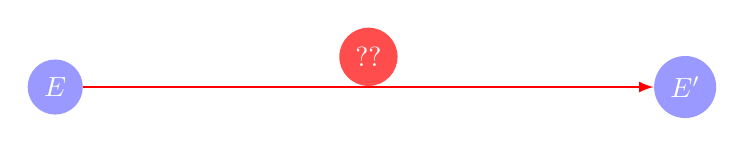
\begin{tikzpicture}
      \path[every node/.style={circle,white,fill=blue!40!white}]
      (0,0) node (E) {$E$}
      (8,0) node (E1) {$E'$};
      \uncover<2->{
        \fill[-latex,red,thick] (E) edge node[above,white,fill=red!70!white,circle] {??} (E1);
      }
    \end{tikzpicture}
  \end{center}
\end{frame}

%%

\begin{frame}[plain]
  \begin{tikzpicture}[overlay,remember picture]
    \draw (current page.center) +(0,1) node[rotate=90]{\includegraphics[height=\paperwidth]{wie-ohr.jpg}};
  \end{tikzpicture}
\end{frame}

%%

\begin{frame}[plain]
  \begin{tikzpicture}[overlay,remember picture]
    \draw
    (current page.center) +(0,-1) node {\includegraphics[width=460px]{pepe_silvia.jpg}}
    +(0,-4) node[white] {\Huge\bf IT'S FUNCTORIAL, BRUH!!1!};
  \end{tikzpicture}
\end{frame}

%%

\begin{frame}
  \Huge\centering
  \begin{tikzpicture}
    \useasboundingbox (-5,-2) -- (5,2);
    \path
    (0,0) node {$\circlearrowright$}
    (-4,0) node {Algebra}
    (4,0) node {Geometry};
  \end{tikzpicture}
\end{frame}

%%

\begin{frame}{Isogenies}
  \large\centering
  \begin{tikzpicture}
    \draw[white,font=\normalsize,
    every node/.style={rounded corners=10,fill=blue!40!white}]
    (0,0) node (E1) {$y^2 = x^3 + 1$}
    (12,0) node (E2) {$y^2 = x^3 - x$}
    (E1) edge[-latex,thick,draw=red] node[circle,fill=red!70!,above] {\Huge $φ$} (E2);

    \draw[every node/.style={anchor=west}]
    (-1,-2) node {Algebraic morphisms:~~~~
      \normalsize $\displaystyle \left(\frac{5x^2 + 5x + 4}{x + 1},\quad y\frac{2x^2 + 4x - 4}{x^2 + 2x + 1}\right)$}
    ++(0,-2) node {Group morphisms:~~~~ \normalsize $φ(P + Q) = φ(P) + φ(Q)$};

    \uncover<2->{
      \path[latex-{Bar[right,scale=3]},thick,
      every node/.style={anchor=west,blue}]
      (9,-3) node {Interpolation} edge +(-7,0)
      ++(0,-2) node {Groups \underline{\bf of} morphisms} edge +(-7,0);
    }
  \end{tikzpicture}
\end{frame}

%%

\begin{frame}{``Classes'' of isogenies}
  \large\centering
  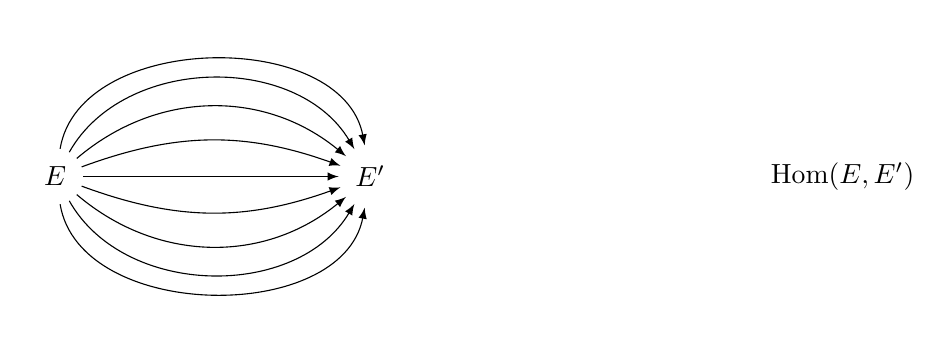
\begin{tikzpicture}
    \fill[circle] (0,0) node(A){$E$} (4,0) node(B){$E'$};
    \foreach  \i in {-4,...,4} {
      \draw[-latex] (A) edge[bend left=\i*20] (B);
    }
    \node at (10,0) {$\Hom(E,E')$};
  \end{tikzpicture}
\end{frame}

%%

\begin{frame}{Degree}
  \begin{columns}
    \begin{column}{0.5\textwidth}
      \centering
      \[\deg(φ) \in ℕ^+\]
      \vspace{1em}
      \begin{itemize}
        \setlength{\itemsep}{2em}
      \item A measure of ``size'';
      \item<2-> \emph{Multiplicative.}
      \end{itemize}
    \end{column}
    \begin{column}{0.5\textwidth}
      \centering
      \begin{tikzpicture}
        \fill[blue!50!white]
        (0,0) circle (1mm) node(A){}
        ++(2,0) circle (1mm) node(B){}
        ++(4,0) circle (1mm) node(C){};
        \draw[-latex,red]
        (A) edge[bend left] node[above]{$φ$} (B)
        (B) edge[bend left] node[above]{$ψ$} (C);

        \uncover<2->{
          \node at (3,-2) {\emph{$\deg(ψ∘φ) = \deg(ψ)\deg(φ)$}};
        }
      \end{tikzpicture}
    \end{column}
  \end{columns}
\end{frame}

%%

\begin{frame}{The larger the degree, the more isogenies}
  \centering\large
  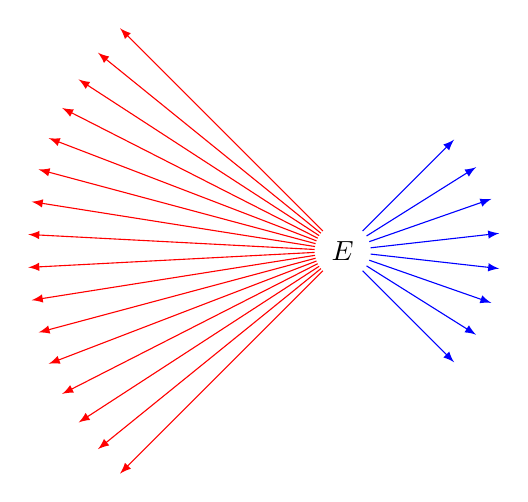
\begin{tikzpicture}
    \draw (0:0) node[circle](A){$E$};
    \foreach  \i in {0,...,7} {
      \draw[blue,-latex] (A) edge (90/7*\i-45:2);
    }
    \foreach  \i in {0,...,15} {
      \draw[red,-latex] (A) edge (90/15*\i-45:-4);
    }
  \end{tikzpicture}
\end{frame}

%% 

\begin{frame}{Lattices of isogenies}
  \centering
  \begin{tikzpicture}
    \node (E1) at (0,0) {$E'$};
    \node (E) at (6,0) {$E$};
    \uncover<2->{
      \draw[dashed,->] (E) edge node[above]
      {$\uncover<3->{\alert{a}}φ+\uncover<3->{\alert{b}}ψ$} (E1);
    }
    
    \draw[->] (E) edge[bend right] node[above] {$φ$} (E1)
    edge[bend left] node[above] {$ψ$} (E1);
    \node at (9,1) {$φ,ψ ∈ \Hom(E,E')$};

    \uncover<2->{
      \node at (10,-1) {$(\uncover<3->{\alert{a}}φ + \uncover<3->{\alert{b}}ψ)(P)
        :=
        \uncover<3->{[\alert{a}]}φ(P) + \uncover<3->{[\alert{b}]}ψ(P)$};
    }
  \end{tikzpicture}

  \bigskip
  
  \uncover<4->{
    \begin{itemize}
      \setlength{\itemsep}{1.5em}
    \item $\deg(aφ) = a^2\deg(φ)$,
    \item $\big\lvert \deg(φ+ψ) - \deg(φ) - \deg(ψ) \big\rvert ≤ 2\sqrt{\deg(φ)\deg(ψ)}$,
    \item $\deg$ is a \emph{positive definite quadratic form.}
    \end{itemize}
  }
\end{frame}

%%

\begin{frame}{Endomorphisms}
  \large
  \begin{columns}
    \begin{column}{0.5\textwidth}
      \centering
      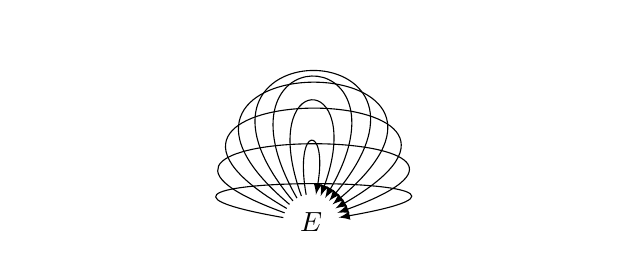
\begin{tikzpicture}
        \fill (0,-1) node[circle](A){$E$};
        \foreach  \i in {1,...,8} {
          \draw[-latex] (A) edge[loop,out=90+10*\i,in=90-10*\i,looseness=20-\i] (A);
        }
      \end{tikzpicture}
    \end{column}
    \begin{column}{0.5\textwidth}
      \[\emph{(φ+ψ)}(P) := φ(P) + ψ(P)\]
      \bigskip
      \[\emph{(φ∘ψ)}(P) := φ(ψ(P))\]
      \bigskip
      \[\emph{φ∘(ψ+χ) = φ∘ψ + φ∘χ}\]
    \end{column}
  \end{columns}
\end{frame}

%%

\begin{frame}{Endomorphism rings}
  \large\centering
  \begin{tikzpicture}
    \node at (-1,0) {$ℚ(\sqrt{-p})$};
    \uncover<2->{
      \node at (1.7,-0.2) {$ℚ(\sqrt{-q})$};
    }
    \uncover<3->{
      \draw (0,-2) ellipse (7cm and 2.5cm);
      \node at (1,-3) {$ℚ(\sqrt{-r})$};
      \node at (-5,-3) {\normalsize $ℚ(\sqrt{-s})$};
      \node at (-1.5,-2.5) {\small $ℚ(\sqrt{-t})$};
      \node at (5,-2) {\small $ℚ(\sqrt{-t})$};
      \node at (0,-1) {\footnotesize $ℚ(\sqrt{-u})$};
      \node at (3,-1.5) {\tiny $ℚ(\sqrt{-v})$};
      \node at (-3,-1) {\normalsize $ℚ(\sqrt{-w})$};
      \node at (4,-3.5) {\small $ℚ(\sqrt{-z})$};
    }

    \uncover<1>{\node at (0,-5) {Quadratic imaginary field};}
    \uncover<2->{\node at (0,-6) {\emph{$i^2 = -p\qquad j^2 = -q\qquad ij = -ji$}};}
    \uncover<3->{\node at (0,-5) {Quaternion algebra};}
  \end{tikzpicture}
\end{frame}

%%

\begin{frame}{Orders}
  \Large
  \begin{columns}
    \begin{column}{0.6\textwidth}
      \[
        \frac{1}{2}
        \begin{pmatrix}
          2 & 0 & 0 & 1\\
          0 & 2 & 1 & 0\\
          0 & 0 & 1 & 0\\
          0 & 0 & 0 & 1 
        \end{pmatrix}
        ~~
        \textcolor{black!50!white}{
          \begin{pmatrix}
            1\\i\\j\\ij
          \end{pmatrix}
        }
      \]
    \end{column}
    \begin{column}{0.4\textwidth}
      \centering
      Order type:
      \[\O \simeq \alpha\O\alpha^{-1}\]
    \end{column}
  \end{columns}
\end{frame}

%%

\begin{frame}
  \centering
  \begin{tikzpicture}
    \useasboundingbox (-2,3) rectangle (12,-4);
    \path[circle]
    (0,-1) node(A){$E_0$}
    (4,-1) node(B){\only<2->{$E$}};

    \foreach  \i in {1,...,8} {
      \draw[-latex] (A) edge[loop,out=90+10*\i,in=90-10*\i,looseness=20-\i] (A);
      \uncover<2->{\draw[-latex,red] (B) edge[bend left=10*\i] (A);}
      \pgfmathtruncatemacro\s{\i+2}
      \uncover<\s->{\draw[-latex] (B) edge[loop,out=90+5*\i,in=90-5*\i,looseness=20-\i] (B);}
    }

    \begin{scope}[shift={(9,0)},scale=0.5]
      \node at (0,-7) {$ℤ[\sqrt{-q}]$};
      \clip (-5.5,-5.5) rectangle (5.5,5.5);
      \draw[black!20!white] (-5,0) -- (5,0) (0,-5) -- (0,5);
      \foreach \i in {-5,-2.5,...,5} {
        \foreach \j in {-5,...,5} {
          \fill[gray] (\j,\i) circle (2pt);
        }
      }
      \uncover<1>{
        \path[latex-] (0,2.5) node[above] {\small $\sqrt{-q}$} edge (0,0)
        (1,0) node[right] {\small $1$} edge (0,0);
      }
      \uncover<2->{
        \path[-latex,red,thick] (0,0) edge (2,5) edge (3,0);
        \foreach \i in {-1,...,1} {
          \foreach \j in {-2,...,2} {
            \fill[red] (\i*2+\j*3,\i*5) circle (4pt);
          }
        }
      }
    \end{scope}
    
    \uncover<12->{
      \begin{scope}[decoration={random steps,segment length=1mm,amplitude=0.1mm},thick]
        \draw[decorate] (4.4,-0.9) -- ++(0.5,-0.2) -- ++(-0.55,-0.2);
        \draw[decorate] (1.8,-2.5) -- ++(0,-1.2) edge +(0.1,0) edge +(0.1,0.05);
        \draw[decorate] (2,-2.5) -- ++(0,-1.2) edge +(0.1,0) edge +(0.1,0.05);
      \end{scope}
    }
  \end{tikzpicture}

  \uncover<11->{
    \begin{center}
      \emph{Deuring:} $\End(E_0)$ sublattices $\leftrightarrow$ homsets $\leftrightarrow$ curves isogenous to $E_0$.
    \end{center}
  }
\end{frame}

%%

\begin{frame}
  \large\centering
  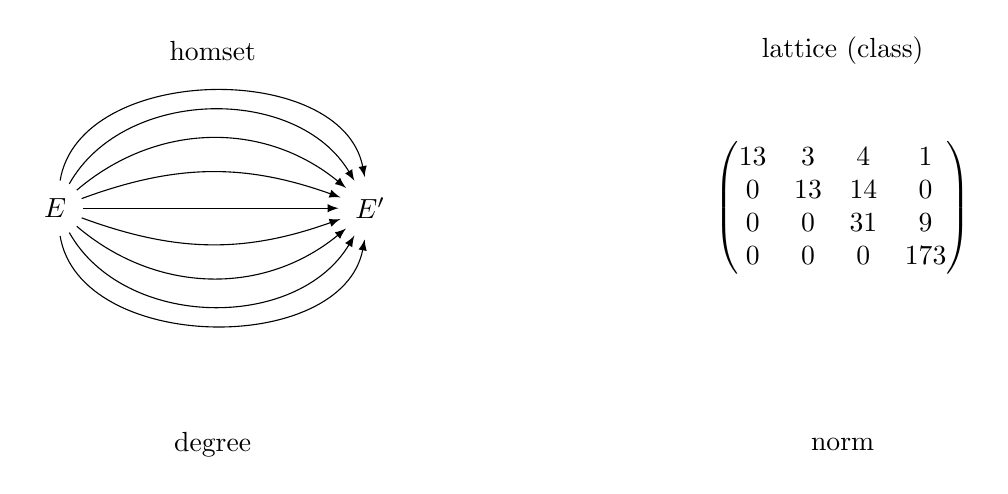
\begin{tikzpicture}
    \node at (2,2) {homset};
    \fill[circle] (0,0) node(A){$E$} (4,0) node(B){$E'$};
    \foreach  \i in {-4,...,4} {
      \draw[-latex] (A) edge[bend left=\i*20] (B);
    }

    \node at (10,2) {lattice (class)};
    \node at (10,0) {$\begin{pmatrix}
        13 & 3 & 4 & 1\\
        0 & 13 & 14 & 0\\
        0 & 0 & 31 & 9\\
        0 & 0 & 0 & 173 
      \end{pmatrix}$
    };
    \uncover<2->{
      \node at (2,-3) {degree};
      \node at (10,-3) {norm};
    }
  \end{tikzpicture}
\end{frame}

%%

\begin{frame}{The supersingular space}
  \large
  \begin{itemize}
    \setlength{\itemsep}{2em}
  \item $\approx \frac{p}{12}$ curves defined over $\F_{p^2}$
  \item of which $\sim \sqrt{p}$ curves defined over $\F_p$
  \item Connected by $\ell$-isogenies for any choice of $\ell > 1$
  \end{itemize}
\end{frame}

%%

\begin{frame}{The endomorphism ring problem}
  \large
  \begin{columns}
    \begin{column}{0.4\textwidth}
      Given a random supersingular curve $E$, compute a basis of
      $\End(E)$.
    \end{column}
    \begin{column}{0.1\textwidth}
      \huge
      \[\Leftrightarrow\]
    \end{column}
    \begin{column}{0.4\textwidth}
      Given random supersingular curves $E, E'$, compute an isogeny
      $E\to E'$.
    \end{column}
  \end{columns}

  \vfill
  \pause
  
  \begin{center}
    Both problems are random self-reducible    
  \end{center}
\end{frame}

%%

\begin{frame}{Collision search: Galbraith}
  \large\centering
  \begin{tikzpicture}
    \coordinate (s) at (0,0);
    \coordinate (e) at (s);
    \foreach \i in {0,...,4} {
      \coordinate (new) at ($(s)+(90+45*rand:1)$);
      \draw[latex-,red] ($(s)+(-0.03,0)$) to ($(new)+(-0.03,0)$);
      \draw[latex-,blue] ($(e)+(0.03,0)$) to ($(new)+(0.03,0)$);
      \coordinate (s) at (new);
      \coordinate (e) at (new);
    }
    \foreach \i in {0,...,6} {
      \draw[latex-,red] (s) to ++(180+45*rand:1) coordinate (s);
      \draw[latex-,blue] (e) to ++(45*rand:1) coordinate (e);
    }
    \draw (s) node[anchor=east]{$E$} (e) node[anchor=west] {$E'$};
  \end{tikzpicture}
\end{frame}

%%

\begin{frame}{Collision search: Delfs-Galbraith}
  \large
  \begin{tikzpicture}[overlay,remember picture]
    \draw (current page.center) ++(4,0)
    node{$\F_p$ subspace} circle (3cm)
    ++(-2.8,0) coordinate (s);
    \foreach \i in {0,...,6} {
      \draw[latex-] (s) to ++(180+45*rand:1) coordinate (s);
    }
    \draw (s) node[anchor=east]{$E$};
    \foreach \j in {-3,-1,...,3} {
      \coordinate (s1) at (s);
      \foreach \i in {0,...,6} {
        \draw[-latex,black!30!white] (s1) to ++(45*rand+\j*30:1) coordinate (s1);
      }
    }
  \end{tikzpicture}
\end{frame}

%%

\begin{frame}{Frobenius}
  \large
  \begin{columns}
    \begin{column}{0.5\textwidth}
      \[
        \begin{aligned}
          E &: y^2 = x^3 + ax + b\\[2em]
          E^{(p)} &: y^2 = x^3 + a^p x + b^p\\
        \end{aligned}
      \]
    \end{column}
    \begin{column}{0.5\textwidth}
      \[
        \begin{aligned}
          \pi : E &→ E^{(p)}\\
          (x,y) &↦ (x^p, y^p)
        \end{aligned}
      \]
    \end{column}
  \end{columns}
\end{frame}

%%

\begin{frame}{Reflections}
  \large\centering
  \begin{tikzpicture}
    \draw (0,1) node{$\F_p$ subspace} (0,0) circle (3cm)
    ++(-2.5,0) node[anchor=west]{$E'$} coordinate (E) coordinate (Ep);
    \foreach \i in {0,...,6} {
      \draw[latex-] (E) to ++(180+25:1) coordinate (E);
      \draw[-latex] (Ep) to ++(180-25:1) coordinate (Ep);
    }
    \draw (E) node(E)[anchor=east]{$E$} (Ep) node(Ep)[anchor=east]{$E^{(p)}$};
    \draw[-latex] (Ep) edge node[left]{$\pi$} (E);
  \end{tikzpicture}  
\end{frame}

%%

\begin{frame}{Geometry of numbers}
  \centering\large
  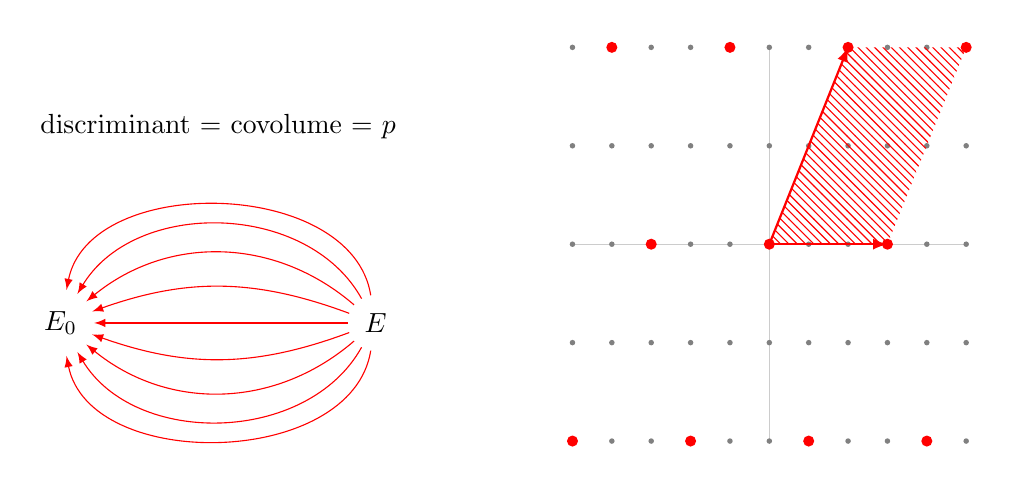
\begin{tikzpicture}
    \path[circle]
    (0,-1) node(A){$E_0$}
    (4,-1) node(B){$E$};

    \foreach  \i in {-4,...,4} {
      \draw[-latex,red] (B) edge[bend left=20*\i] (A);
    }

    \node at (2,1.5) {discriminant = covolume = $p$};
    
    \begin{scope}[shift={(9,0)},scale=0.5]
      \clip (-5.5,-5.5) rectangle (5.5,5.5);
      \draw[black!20!white] (-5,0) -- (5,0) (0,-5) -- (0,5);
      \foreach \i in {-5,-2.5,...,5} {
        \foreach \j in {-5,...,5} {
          \fill[gray] (\j,\i) circle (2pt);
        }
      }
      \path[-latex,red,thick] (0,0) edge (2,5) edge (3,0);
      \foreach \i in {-1,...,1} {
        \foreach \j in {-2,...,2} {
          \fill[red] (\i*2+\j*3,\i*5) circle (4pt);
        }
      }
      \fill[pattern color=red,pattern=north west lines] (0,0) -- (2,5) -- (5,5) -- (3,0);
    \end{scope}
  \end{tikzpicture}

  \bigskip
  
  Gaussian heuristic $⇒ d_1 ≈ d_2 ≈ d_3 ≈ d_4 ≈ \sqrt{p}$
\end{frame}

%%

\begin{frame}{Squared minima of random $\Hom(E,E')$, log scale}
  \centering
  \begin{tikzpicture}
    \draw
    (0,0) node{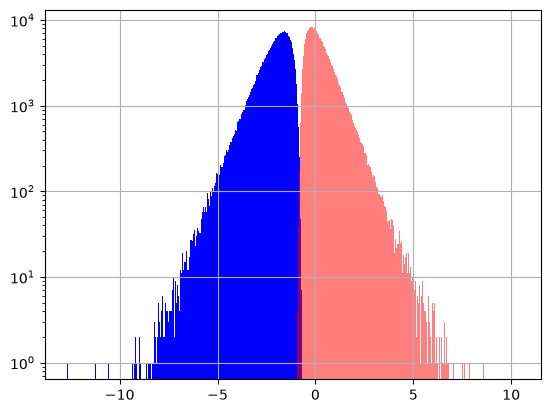
\includegraphics[width=0.47\textwidth]{hom_d1,4.png}}
    +(0,-3) node{1st and 4th minimum}
    (8,0) node{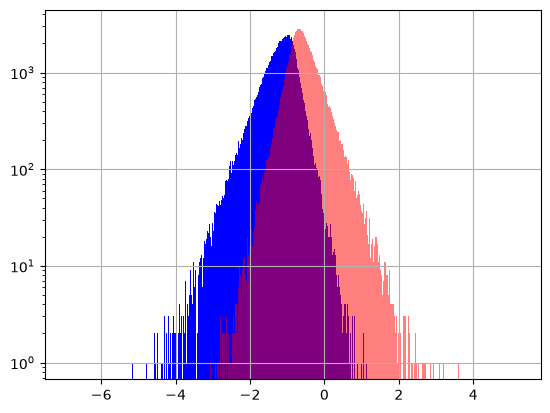
\includegraphics[width=0.47\textwidth]{hom_d2,3.png}}
    +(0,-3) node{2nd and 3rd minimum};
  \end{tikzpicture}
\end{frame}

%%

\begin{frame}{How hard is it to find a short isogeny?}
  \large\centering
  \begin{tikzpicture}
    \node (E) at (0,0) {$E$};
    \node (E1) at (10,0) {$E'$};

    \uncover<1>{
      \draw[-latex] (E) edge node[above]{$\deg φ ≈ \sqrt{p}$} (E1);
    }
    \uncover<2->{
      \draw ($(E)!0.5!(E1)$) edge[latex-] node[above]{$p^{1/4}$} (E) edge[latex-] node[above]{$p^{1/4}$} (E1);
    }
  \end{tikzpicture}

  \bigskip
  
  \begin{itemize}
    \setlength{\itemsep}{1em}
  \item $O(n)$ isogenies of degree $n$ from $E$
  \item $⇒$ $O(n^2)$ isogenies of degree $≤ n$ from $E$
  \item<2-> $⇒$ If we're lucky, we can meet-in-the-middle at cost
    $O(\sqrt{p})$.
  \end{itemize}
\end{frame}

%%

\begin{frame}{Minima of endomorphism rings}
  \centering
  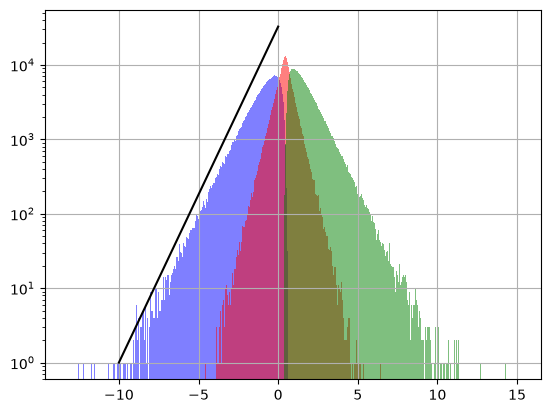
\includegraphics[height=0.85\textheight]{end_d1-3.png}
\end{frame}

%%

\begin{frame}{Duality}
  \Large\centering
  \begin{tikzpicture}
    \node (pp) at (-4,0) {$\Hom(E_1,E_2)$};
    \node (dd) at (4,0) {$\Hom(E_1^{(p)},E_2^{(p)})$};
    \node (pd) at (0,3) {$\Hom(E_1^{(p)},E_2)$};
    \node (dp) at (0,-3) {$\Hom(E_1,E_2^{(p)})$};

    \draw
    ($(pp)!0.5!(dd)$) node{$\#$}
    ($(pp)!0.5!(dp)$) node[rotate=45]{$\perp$}
    ($(pp)!0.5!(pd)$) node[rotate=-45]{$\perp$}
    ($(dd)!0.5!(dp)$) node[rotate=135]{$\perp$}
    ($(dd)!0.5!(pd)$) node[rotate=-135]{$\perp$};
    
  \end{tikzpicture}
\end{frame}

%%

\begin{frame}{Transference}
  \begin{tikzpicture}
    \draw
    (0,0) node {$\Hom(E_1,E_2)$}
    +(0,-1) node {$d_1,d_2,d_3,d_4$}
    ++(4,0) node {$\Hom(E_1,E_2^{(p)})$}
    +(0,-1) node {$d_1^*,d_2^*,d_3^*,d_4^*$}
    ++(6,-0.5) node {$d_1d_4^* ≈ d_2d_3^* ≈ d_3d_2^* ≈ d_4d_1^* ≈ p$};
    
    \uncover<2->{
      \draw
      (0,-3) node {$\End(E)$}
      +(0,-1) node {$1,d_1,d_2,d_3$}
      ++(4,0) node {$\Hom(E,E^{(p)})$}
      +(0,-1) node {$d_1^*,d_2^*,d_3^*,d_4^*$}
      ++(6,-0.5) node {$d_4^* ≈ d_2d_3^* ≈ d_3d_2^* ≈ d_4d_1^* ≈ p$};
    }
  \end{tikzpicture}
\end{frame}

%%

\begin{frame}{Wesolowski's attack}
  \large\centering
  \begin{tikzpicture}
    \node (E) at (0,0) {$E$};
    \node (E1) at (10,0) {$E^{(p)}$};

    \uncover<1>{
      \draw[-latex] (E) edge node[above]{$p^{1/3}$} (E1);
    }
    \uncover<2->{
      \draw ($(E)!0.5!(E1)$) edge[latex-] node[above]{$p^{1/6}$} (E) edge[latex-] node[above]{$p^{1/6}$} (E1);
    }
    \uncover<3->{
      \draw (E1) edge[bend left] node[below]{$π$} (E);
    }
  \end{tikzpicture}

  \bigskip
  
  \begin{itemize}
    \setlength{\itemsep}{1em}
  \item $O(n)$ isogenies of degree $n$ from $E$
  \item $⇒$ $O(n^2)$ isogenies of degree $≤ n$ from $E$
  \item<2-> $⇒$ If we're lucky, we can meet-in-the-middle at cost
    $O(p^{1/3})$.
  \end{itemize}
\end{frame}

%%


\begin{frame}[plain]
  \centering
  \begin{tikzpicture}[remember picture,overlay]
    \begin{scope}[xscale=1.7,yshift=-15,opacity=0.8]
      \def\crater{12}
      \def\jumpa{-8}
      \def\jumpb{9}
      \def\diam{5cm}

      \foreach \i in {1,...,\crater} {
        \draw[blue] (360/\crater*\i : \diam) to[bend right] (360/\crater*\i+360/\crater : \diam);
        \draw[red] (360/\crater*\i : \diam) to[bend right] (360/\crater*\i+\jumpa*360/\crater : \diam);
        \draw[green] (360/\crater*\i : \diam) to[bend right=50] (360/\crater*\i+\jumpb*360/\crater : \diam);
      }
    \end{scope}
    
    \draw (0,0.5) node{\Huge\bf Thank you};
    \draw (0,-0.6) node{\large\url{https://defeo.lu/}};
    \draw (0,-1.3) node{\large\includegraphics[height=0.9em]{mastodon.png}~\href{https://twitter.com/luca_defeo}{@luca\_defeo@ioc.exchange}};
    \draw (0,-1.9) node{\large\includegraphics[height=0.9em]{bluesky.png}~\href{https://bsky.app/profile/bsky.defeo.lu}{@bsky.defeo.lu}};
  \end{tikzpicture}
\end{frame}

\end{document}


% LocalWords:  Isogeny abelian isogenies hyperelliptic supersingular Frobenius
% LocalWords:  isogenous
